\documentclass[12pt]{article}
\usepackage[margin=1in]{geometry} 
\usepackage{amsmath,amsthm,amssymb,amsfonts}
\usepackage{enumitem}
\usepackage{tabu}
\usepackage{xcolor}
\usepackage{mathtools}
\usepackage{tcolorbox} 
\usepackage{changepage} 
\usepackage{kpfonts}
\usepackage{picture}
\usepackage{venndiagram}
\usepackage{graphicx}

\newcommand{\prob}[1]{\mathbb{P}(#1)}
\newcommand{\condprob}[2]{\mathbb{P}(#1 \text{ } \lvert \text{ } #2)}
\newcommand{\expected}[1]{\text{E}(#1)}
\newcommand{\variance}[1]{\text{V}(#1)}

\newcommand{\N}{\mathbb{N}}
\newcommand{\Z}{\mathbb{Z}}
\newcommand{\R}{\mathbb{R}}
\newcommand{\field}{\mathcal{F}}

\begin{document}
% ===================================================================================
% ===================================================================================

\section*{CHAPTER 8: Law of Large Numbers}
% ================ SECTION 8.1 ================
\subsection*{Law of Large Numbers for Discrete Random Variables}
\noindent
We have also defined probability mathematically as a value of a distribution function for the random variable representing the experiment. The Law of Large Numbers, which is a theorem proved about the mathematical model of probability, shows that this model is consistent with the frequency interpretation of  probability.

\subsubsection*{ChebyShev Inequality}
\noindent
\textbf{Theorem 8.1 (ChebyShev Inequality)} Let $X$ be a discrete random variable with expected value $\mu \expected{X}$, and let $\epsilon > 0$ be any positive real number. Then,

\begin{equation*}
\prob{\lvert X - \mu \rvert \geq \epsilon} \leq \frac{\variance{X}}{\epsilon^2}.
\end{equation*}

\begin{tcolorbox}
\noindent
Let X by any random variable with $\expected{X} = \mu$ and $\variance{X} = \sigma^2$. Then, if $\epsilon = k \sigma$, Chebyshev's Inequality states that

\begin{equation*}
\prob{\lvert X - \mu \rvert \geq k \sigma} \leq \frac{\sigma^2}{k^2 \sigma^2} = \frac{1}{k^2}.
\end{equation*}

\noindent
Thus, for any random variable, the probability of a deviation from the mean of
more than k standard deviations is $\leq \frac{1}{k^2}$. If, for example, $k = 5$, $\frac{1}{k^2} = .04$.

\vspace*{.5cm}
\noindent
Chebyshev’s Inequality is the best possible inequality in the sense that, for any
$\epsilon > 0$, it is possible to give an example of a random variable for which Chebyshev’s Inequality is in fact an equality. To see this, given $\epsilon > 0$, choose X with distribution 

\begin{equation*}
p_X = {- \epsilon \qquad  + \epsilon \choose 1/2 \qquad 1/2}
\end{equation*}

Then $\expected{X} = 0$, $\variance{X} = \epsilon^2$, and 

\begin{equation*}
\prob{\lvert X - \mu \rvert \geq \epsilon} \leq \frac{\variance{X}}{\epsilon^2} = 1.
\end{equation*}

We are now prepared to state and prove the Law of Large Numbers.
\end{tcolorbox}

% https://www.youtube.com/watch?v=uMgK000XFhA
\noindent
Alternatively, Chebyshev's theorem says that the proportion of any distribution that lies within $k$ standard deviations of the mean is at least: $1-\frac{1}{k^2}$, where $k$ is any positive number greater than $1$. This theorem applies to \textbf{all distributions}.

\begin{tcolorbox}
For example, Chebyshev's theorem says that within $2$ standard deviations of the mean, you will find at least

\begin{equation*}
1 - \frac{1}{k^2} = 1 - \frac{1}{2^2} = 1 - \frac{1}{4} = \frac{3}{4},
\end{equation*} 

\noindent
or at least $75\%$ of data will lie within $2$ standard deviations from the mean.
\end{tcolorbox}

\vspace*{.5cm}
\begin{tcolorbox}
Let $X_1, X_2, \ldots, X_n$ be a Bernoulli trials process with probability $.3$ for success and $.7$ for failure. Then, $\expected{X_j} = .3$ and $\variance{X_j} = .3 \cdot .7 = .21$. If

\begin{equation*}
A_n = \frac{S_n}{n} = \frac{X_1, X_2, \ldots, X_n}{n}
\end{equation*}

\noindent
is the average of the $X_j$, then $\expected{A_n} = .3$ and $\variance{A_n} = \frac{\variance{S_n}}{n^2} = \frac{.21}{n}$. 

\vspace*{.3cm}
\noindent
Let $\epsilon = .1$. Then, Chebyshev's Inequality states that 

\begin{equation*}
\prob{\lvert A_n - .3 \rvert \geq .1 } \leq \frac{.21}{n(.1)^2} = \frac{21}{n}.
\end{equation*}

\noindent
If $n = 100$, this can be rewritten as 

\begin{equation*}
\prob{.2 <  A_{100} < .4 } \geq \mathbb{P}_{A_{100}}
\end{equation*}

\noindent
where $\mathbb{P}_{A_{100}}$ is the probability that the mean of $A_n$ lies between $.2$ and $.4$, which is $.1$ away from $\expected{A_n} = .3$. By Chebyshev, we can calculate this by finding how many standard deviations $.1$ is. The standard deviation, $\sigma = \sqrt{\frac{.21}{100}} = .0458$. Thus, $k = \frac{.1}{.0458} = 2.182$. Thus, 

\begin{equation*}
\mathbb{P}_{A_{100}} = 1 - \frac{1}{2.182^2} = .79 = 79\%.
\end{equation*}
\end{tcolorbox}

\subsubsection*{Law of Large Numbers}
\noindent
\textbf{Theorem 8.2: Law of Large Numbers} Let $X_1, X_2, \ldots, X_n$ be an independent trial process, with finite expected value $\mu = \expected{X_j}$, and finite variance $\sigma = \variance{X_j}$. Then for any $\epsilon > 0$,

\begin{equation*}
\mathbb{P} \Bigg ( \Bigg \lvert \frac{S_n}{n} - \mu \Bigg \rvert \geq \epsilon \Bigg ) \rightarrow 0
\end{equation*}

\noindent
as $n \rightarrow \infty$. Equivalently,

\begin{equation*}
\mathbb{P} \Bigg ( \Bigg \lvert \frac{S_n}{n} - \mu \Bigg \rvert < \epsilon \Bigg ) \rightarrow 1
\end{equation*}

\noindent
as $n \rightarrow \infty$. 

\begin{center}
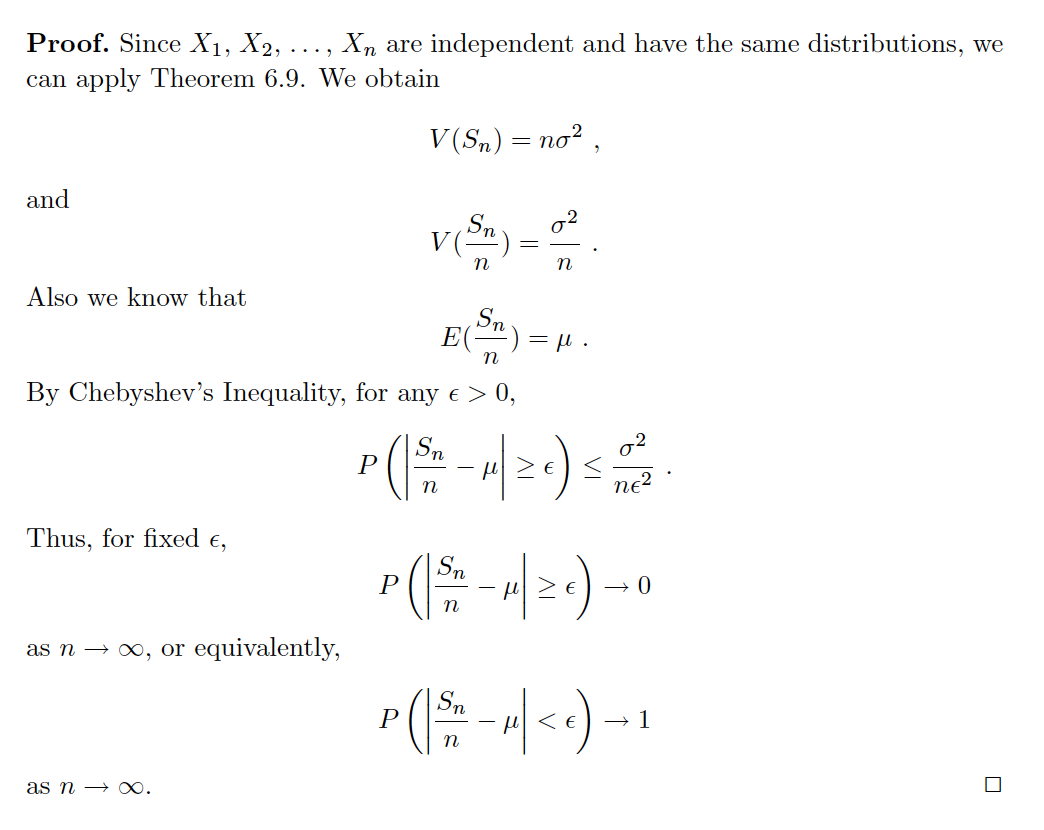
\includegraphics[width=13cm, height=10cm]{LLN_proof_pic}
\end{center}

% https://www.youtube.com/watch?v=MntX3zWNWec
\noindent
The \textbf{Law of Large Numbers} states that as the number of observations increases, the actual or observed probability approaches the theoretical or expected probabilities. 

\vspace*{.3cm}
\noindent
\textbf{Weak Law of Large Numbers} vs. \textbf{Strong Law of Large Numbers} \\
\noindent
The \textbf{WLLN} says that for a large sample, there is a very high probability that the mean of the sample will be very close to the expected value, due to \textit{weak convergence}. However, the probability of convergence is still very high.

\vspace*{.3cm}
\noindent
The \textbf{SLLN} says that for a large sample, the mean of the sample will almost surely be the expected value, due to \textit{strong convergence}. The proof of the \textbf{SLLN} is much more complex and much harder to prove.

\begin{center}
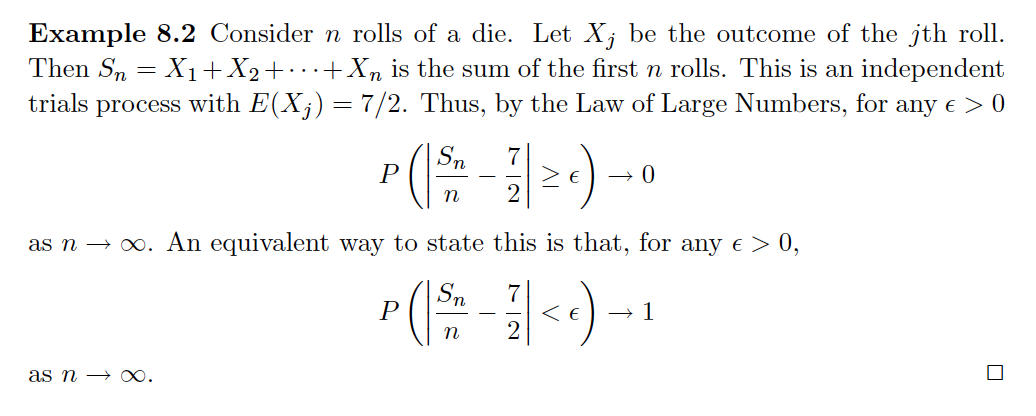
\includegraphics[width=13cm, height=6cm]{DIE_ROLLING_EXAMPLE}
\end{center}

\noindent
There are exercises for \textbf{LLN} on page $312$.

% ================ SECTION 8.2 ================

\subsection*{Law of Large Numbers for Discrete Random Variables}
This law has a natural analogue for continuous probability distributions, which we consider somewhat more briefly here.

\subsubsection*{ChebyShev Inequality}
\noindent
\textbf{Theorem 8.3 (ChebyShev Inequality)} Let $X$ be a continuous random variable with density function $f(x)$. Suppose $X$ has a finite expected value $\mu \expected{X}$ and finite variance $\variance{X} = \sigma^2$. Then, for any positive number $\epsilon > 0$ we have

\begin{equation*}
\prob{\lvert X - \mu \rvert \geq \epsilon} \leq \frac{\variance{X}}{\epsilon^2}.
\end{equation*}

\noindent
Note that this theorem says nothing if $\variance{X} = \sigma^2$ is infinite.

\subsubsection*{Law of Large Numbers}
\noindent
\textbf{Theorem 8.4: Law of Large Numbers} Let $X_1, X_2, \ldots, X_n$ be an independent trial process with a continuous density function $f$, finite expected value $\mu$, and finite variance $\sigma^2$. Let $S_n = X_1, X_2, \ldots, X_n$ be the sum of the $X_i$. Then for any real number $\epsilon > 0$ we have

\begin{equation*}
\lim_{n \rightarrow \infty} \mathbb{P} \Bigg ( \Bigg \lvert \frac{S_n}{n} - \mu \Bigg \rvert \geq \epsilon \Bigg ) = 0,
\end{equation*}

\noindent
or equivalently,

\begin{equation*}
\lim_{n \rightarrow \infty} \mathbb{P} \Bigg ( \Bigg \lvert \frac{S_n}{n} - \mu \Bigg \rvert < \epsilon \Bigg ) = 1.
\end{equation*}

\noindent
There are exercises for \textbf{LLN} on page $320$.

% ========================================================
% ========================================================

\section*{CHAPTER 9: Central Limit Theorem}
\subsubsection*{Central Limit Theorem for Bernoulli Trials}
\noindent
The second fundamental theorem of probability is the \textit{Central Limit Theorem}. This theorem says that if Sn is the sum of n mutually independent random variables, then the distribution function of Sn is well-approximated by a certain type of continuous function known as a normal density function, which is given by the formula

\begin{equation*}
f_{\mu, \sigma} = \frac{1}{\sqrt{2 \pi} \sigma} e^{-(x - \mu)^2 / (2 \sigma^2)}.
\end{equation*}

In this section, we will deal only with the case that $\mu = 0$ and $\sigma = 1$. We will call this particular normal density function the standard normal density, and we will denote it by $\phi (x)$: 

\begin{equation*}
\phi (x) = \frac{1}{\sqrt{2 \pi}} e^{-x^2 / 2}.
\end{equation*}

\noindent
\textbf{Definition 9.1} The \textit{standardized sum} of $S_n$ is given by 

\begin{equation*}
S_n^* = \frac{S_n - np}{\sqrt{npq}},
\end{equation*}

\noindent
where $S_n^*$ has expected value $0$ and variance $1$.

\vspace*{.3cm}
\noindent
\textbf{Approximating Binomial Distributions}
\noindent
We can approximate a binomial distribution function as follows

\begin{align*}
b(n,p,j) &\sim \frac{\phi(x)}{\sqrt{npq}} \\
&= \frac{1}{\sqrt{npq}} \phi \Bigg ( \frac{j - np}{\sqrt{npq}} \Bigg ).
\end{align*}

\noindent
An example of a situation where this can be used is when there are $100$ flips of a fair coin and we want to know the probability of seeing exactly $55$ heads.

%\begin{tcolorbox}
%\end{tcolorbox}
\end{document} 